\section{Pivot Point}
\label{sec:1PPV}

Pivot Point - Jest to matematyczna formuła wyznaczania poziomów wsparć i oporu weryfikując maksima oraz minima występujące w danym okresie. Jest to wzór określający potencjalny zasięg ruchu notowań w danej jednostce czasu. Opiera się na obliczeniu danych za pomocą następujących wzorów: 1, 2, 3, 4 oraz 5.
\begin{equation}
P(Pivot point) = \frac{(H + L + C)}{3}
\label{wzor_1}
\end{equation}
\begin{equation}
R1(Pierwszy opór) = 2*P - L
\label{wzor_2}
\end{equation}
\begin{equation}
S1 (Pierwsze wsparcie) = 2P - H
\label{wzor_3}
\end{equation}
\begin{equation}
R2 (Drugi opór) = P + (R1 - S1)
\label{wzor_4}
\end{equation}
\begin{equation}
S2 (Drugie wsparcie) = P - (R1 - S1)
\label{wzor_5}
\end{equation}


\noindent Do podstawowych własności wskaźnika należą:
\begin{itemize}
\item służą do wyznaczania punktów wsparcia i oporu na rynkach
\item określenie punktu zawarcia transakcji poprzez odpowiednie przecięcia linii
\item ustalenie poziomu oporu branego pod uwagę (pierwszy lub drugi)
\end{itemize}

Najważniejszą własnością opisywanego wskaźnika, stosowaną przy implementacjach strategii, jest fakt wskazywania momentów w których powinny zostać zawarte transakcje. W wypadku Pivot Point należy określić punkt zawarcia transakcji. Na potrzeby programu trzymano się strategii gdzie:
\begin{itemize}
\item sygnałem kupna jest przecięcie linii R1
\item sygnałem sprzedaży jest przecięcie linii S1
\newline
\end{itemize}
\noindent Poniższy listing przedstawia zaimplementowaną strategię w środowisku MATLAB.
\begin{scriptsize}
\begin{lstlisting}
paramSectionLearn = C(1:5400,:);
paramSectionTest = C(5401:end,:);

[m,n]=size(paramSectionLearn);

O=paramSectionLearn(:,1);
L=paramSectionLearn(:,3);
H=paramSectionLearn(:,2);
C=paramSectionLearn(:,4);

%Parametry 
pip = 0.01; % wielkosc pipsa na danym rynku
spread = 1.8 * pip; % spread dla rynku
% pip =1; % wielkosc pipsa na danym rynku

bestReturn = -100;
bestMa = 0;
%Część ucząca

countCandleLearn=m;
lastCandleLearn=0;
krok=1;
%Część valid

paramALengthT=0;
countCandleTest=m1;
lastCandleTest=0;
chwi=1;
tmp=countCandleLearn-1;

P = (H + L + C) / 3;
R1 = 2*P - L;
S1 = 2*P - H;

sumRa=zeros(1,tmp);
Ra=zeros(1,tmp);
lastCandleLearn=tmp;
   
WinReturn=0;
DownReturn=0;
CalmarLearn=0;
BestCalLearn=0;
for paramALengthL=10:100 %liczba świec wstecz ( do max)
    chwi=chwi;

paramZakrespocz(chwi)=paramALengthL;
       
    %-------------obliczanie zysków

    
    for j=2:lastCandleLearn
        
        if R1(j)>C(j) && R1(j)<=C(j-1)
            Ra(j)=C(j+krok)-O(j+1)-spread ;% zysk z j-tej pozycji long zamykanej na zamknięciu po 1 kroku 
        else if S1(j)<C(j) && S1(j)>=C(j-1)
             Ra(j)=-C(j+krok)+O(j+1)+spread   ; 
            end
        end

        sumRa(j)=sumRa(j-1)+Ra(j); %krzywa narastania kapitału
        
        if sumRa(j)>WinReturn
            WinReturn=sumRa(j);
        end
        
        DownReturnTmp=sumRa(j)-WinReturn;
        if  DownReturnTmp<DownReturn
            DownReturn= DownReturnTmp;
        end
     
    end
    chwi=chwi+1;
 sumFinal=sumRa(lastCandleLearn);   
    if bestReturn < sumFinal
    bestMa=paramALengthL;
 end
end

CalmarLearn=-sumFinal/DownReturn;
\end{lstlisting}
\end{scriptsize}

Na podstawie zebranych informacji dotyczących wskaźnika Pivot Point, stworzono powyższy program uwzględniając pozycje sprzedaży i kupna przy określonych przecięciach. Badania przeprowadzono na rynku usdjpy.
\begin{itemize}
\item sygnałem kupna jest przecięcie linii R1
\item sygnałem sprzedaży jest przecięcie linii S1
\newline
\end{itemize}
Podczas badania wskaźnika cały zbiór danych (świec) podzielony został na dwie części: uczącą ($60\%$ całości) oraz testową ($40\%$ całości). W przeprowadzonych badaniach poszukiwano optymalnej wartości parametru $k$ na okresie uczącym, następnie weryfikowano otrzymane wyniki na okresie testowym. Wybór optymalnej wartości parametru (dla czystego wskaźnika Ma) polegał na wyszukaniu najlepszego zysku. \\

\noindent \textbf{\\Wyniki badań przy maksymalizacji po zysku.}\\
\begin{figure}[h!]
\centering
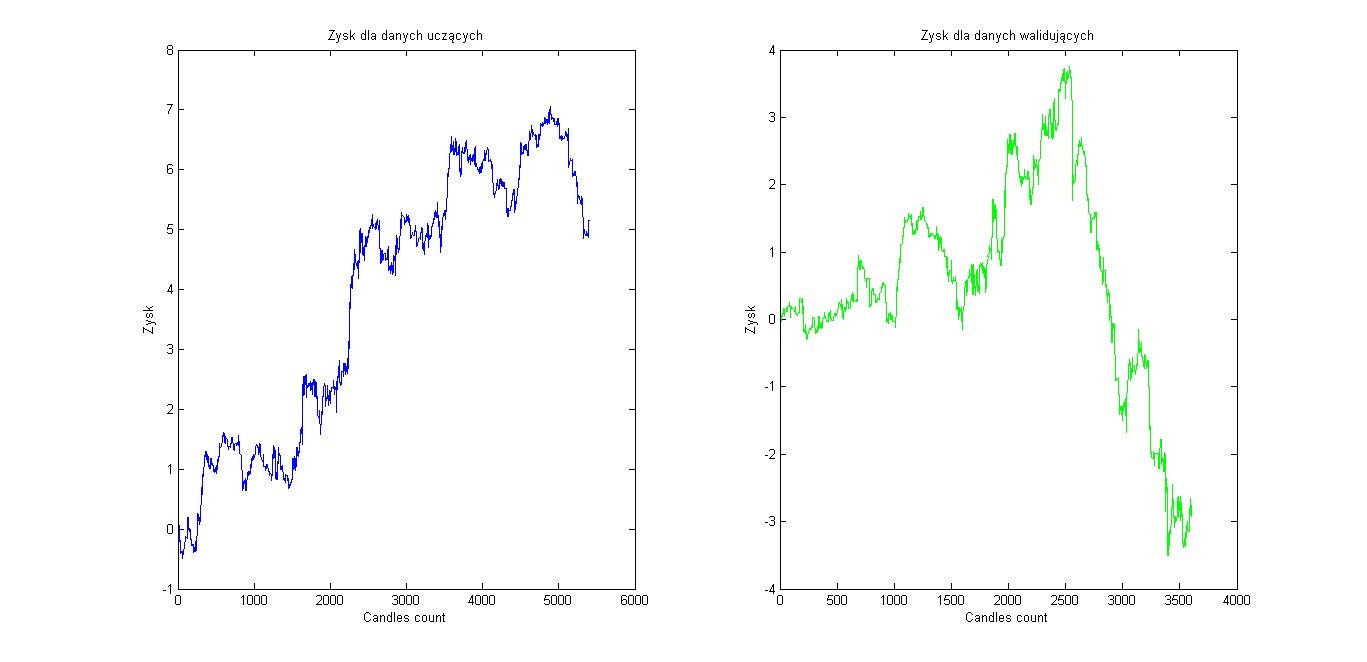
\includegraphics[scale=0.4]{pp_zysk_us.png}
\caption{Zysk}

\end{figure}
\FloatBarrier

\newpage
\noindent \textbf{Wycinek R1 i S1}\\
\begin{figure}[h!]
\centering
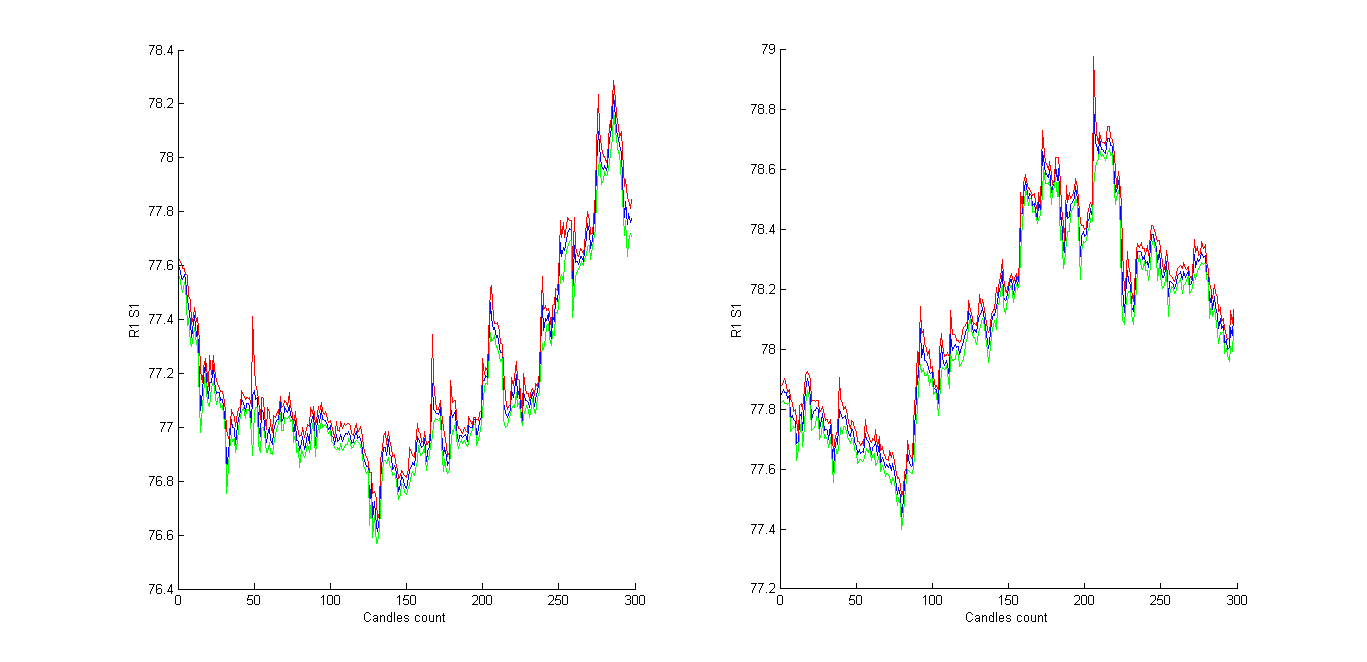
\includegraphics[scale=0.4]{pp_rs_us.png}
\caption{Trend rynku - kolor niebieskim, R1 - kolor czerwony oraz S1 - kolor zielony }
\end{figure}
\FloatBarrier
%
